% Generated by extension/perturbation/make_assets.py. Do not edit.
\definecolor{heldcol}{HTML}{217D91}
\definecolor{ntcol}{HTML}{C9803A}
\definecolor{donorcol}{HTML}{5D6670}
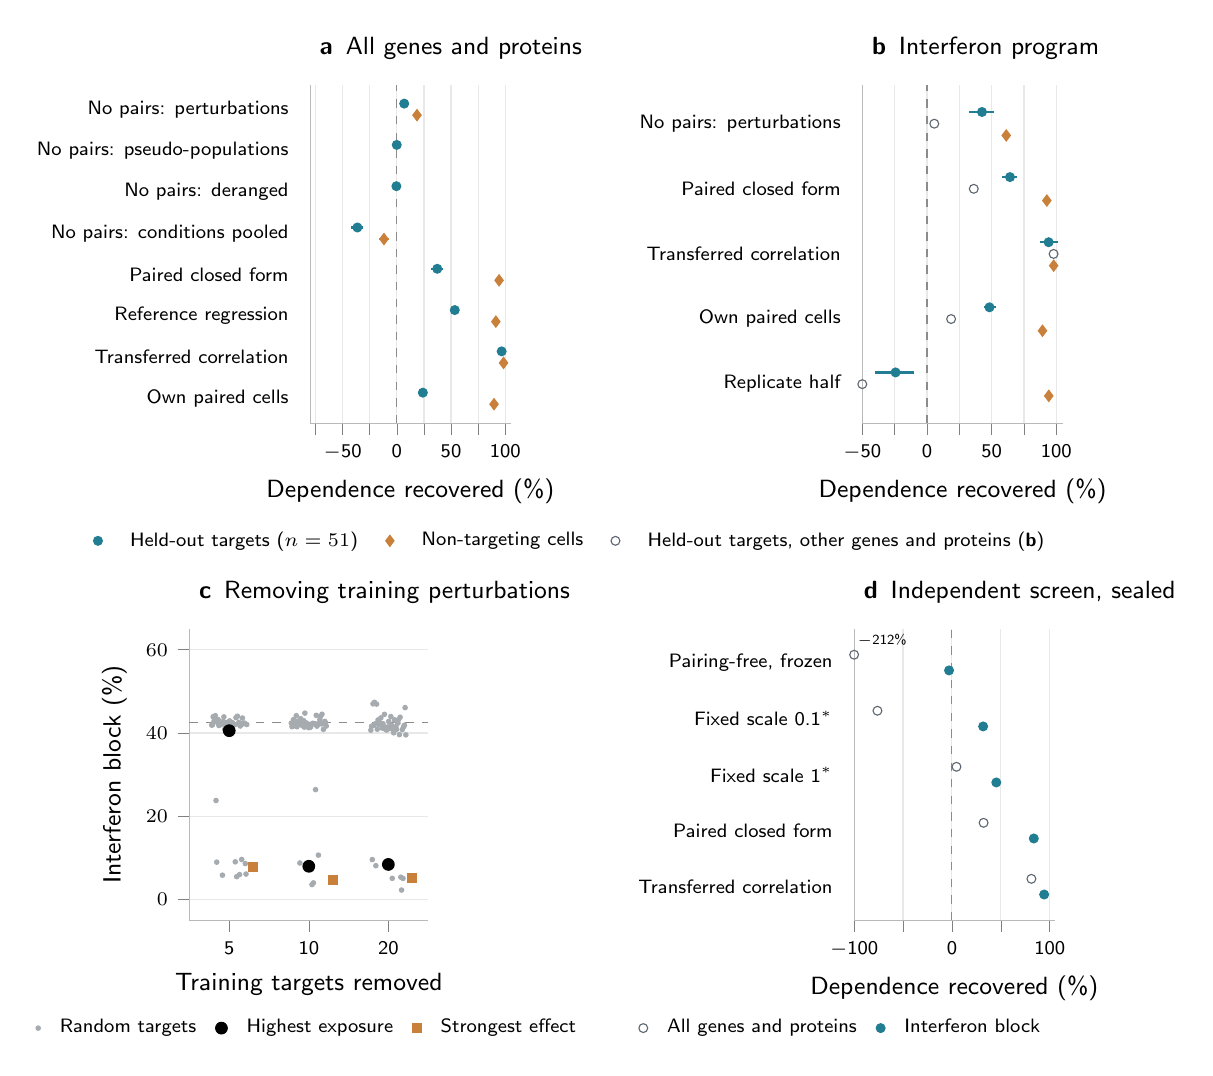
\begin{tikzpicture}[font=\sffamily]
\begin{axis}[name=a,scale only axis,width=.21\textwidth,height=4.3cm,xmin=-80,xmax=105,ymin=.4,ymax=8.6,
 xtick={-75,-50,-25,0,25,50,75,100},xticklabels={,$-$50,,0,,50,,100},ytick={1,...,8},
 yticklabels={{Own paired cells},{Transferred correlation},{Reference regression},{Paired closed form},{No pairs: conditions pooled},{No pairs: deranged},{No pairs: pseudo-populations},{No pairs: perturbations}},
 xlabel={Dependence recovered (\%)},
 title={\textbf{a}\enspace All genes and proteins},
 axis x line*=bottom,axis y line*=left,tick align=outside,y tick style={draw=none},xmajorgrids=true,grid style={gray!18},axis line style={gray!55},tick label style={font=\sffamily\scriptsize},label style={font=\sffamily\small},clip=false,title style={font=\sffamily\small,at={(0,1)},anchor=base west,yshift=5pt}]
\draw[dashed,black!45] (axis cs:0,.4) -- (axis cs:0,8.6);
\draw[heldcol,line width=.8pt] (axis cs:19.80,1.1400000000000001) -- (axis cs:27.75,1.1400000000000001);
\draw[ntcol,line width=.8pt] (axis cs:88.09,0.86) -- (axis cs:91.10,0.86);
\draw[heldcol,line width=.8pt] (axis cs:92.67,2.14) -- (axis cs:100.69,2.14);
\draw[ntcol,line width=.8pt] (axis cs:97.04,1.8599999999999999) -- (axis cs:99.83,1.8599999999999999);
\draw[heldcol,line width=.8pt] (axis cs:49.39,3.14) -- (axis cs:57.18,3.14);
\draw[ntcol,line width=.8pt] (axis cs:89.65,2.86) -- (axis cs:92.90,2.86);
\draw[heldcol,line width=.8pt] (axis cs:31.65,4.14) -- (axis cs:42.22,4.14);
\draw[ntcol,line width=.8pt] (axis cs:92.84,3.86) -- (axis cs:95.72,3.86);
\draw[heldcol,line width=.8pt] (axis cs:-41.96,5.14) -- (axis cs:-31.65,5.14);
\draw[ntcol,line width=.8pt] (axis cs:-16.15,4.86) -- (axis cs:-7.67,4.86);
\draw[heldcol,line width=.8pt] (axis cs:-0.57,6.14) -- (axis cs:-0.27,6.14);
\draw[heldcol,line width=.8pt] (axis cs:-0.15,7.14) -- (axis cs:-0.06,7.14);
\draw[heldcol,line width=.8pt] (axis cs:4.05,8.14) -- (axis cs:9.42,8.14);
\draw[ntcol,line width=.8pt] (axis cs:16.12,7.86) -- (axis cs:21.07,7.86);
\addplot[only marks,mark=*,mark size=1.6pt,color=heldcol] coordinates { (24.00,1.1400000000000001) (96.70,2.14) (53.44,3.14) (37.27,4.14) (-36.41,5.14) (-0.41,6.14) (-0.10,7.14) (6.79,8.14) };
\addplot[only marks,mark=diamond*,mark size=2pt,color=ntcol] coordinates { (89.67,0.86) (98.46,1.8599999999999999) (91.34,2.86) (94.31,3.86) (-11.90,4.86) (18.60,7.86) };
\end{axis}
\begin{axis}[at={(a.outer north east)},anchor=outer north west,xshift=.5cm,name=b,scale only axis,
 width=.21\textwidth,height=4.3cm,xmin=-50,xmax=105,ymin=.4,ymax=5.6,
 xtick={-50,-25,0,25,50,75,100},xticklabels={$-$50,,0,,50,,100},
 ytick={1,2,3,4,5},
 yticklabels={{Replicate half},{Own paired cells},{Transferred correlation},{Paired closed form},{No pairs: perturbations}},
 xlabel={Dependence recovered (\%)},title={\textbf{b}\enspace Interferon program},
 axis x line*=bottom,axis y line*=left,tick align=outside,y tick style={draw=none},xmajorgrids=true,grid style={gray!18},axis line style={gray!55},tick label style={font=\sffamily\scriptsize},label style={font=\sffamily\small},clip=false,title style={font=\sffamily\small,at={(0,1)},anchor=base west,yshift=5pt}]
\draw[dashed,black!45] (axis cs:0,.4) -- (axis cs:0,5.6);
\draw[heldcol,line width=.8pt] (axis cs:-39.82,1.18) -- (axis cs:-10.21,1.18);
\draw[heldcol,line width=.8pt] (axis cs:43.96,2.18) -- (axis cs:53.20,2.18);
\draw[heldcol,line width=.8pt] (axis cs:87.74,3.18) -- (axis cs:101.51,3.18);
\draw[heldcol,line width=.8pt] (axis cs:58.30,4.18) -- (axis cs:69.92,4.18);
\draw[heldcol,line width=.8pt] (axis cs:32.37,5.18) -- (axis cs:51.44,5.18);
\addplot[only marks,mark=*,mark size=1.6pt,color=heldcol] coordinates { (-24.28,1.18) (48.33,2.18) (94.05,3.18) (64.17,4.18) (42.52,5.18) };
\addplot[only marks,mark=o,mark size=1.6pt,color=donorcol] coordinates { (-50.00,1) (18.66,2) (97.87,3) (36.17,4) (5.66,5) };
\addplot[only marks,mark=diamond*,mark size=2pt,color=ntcol] coordinates { (94.16,0.8200000000000001) (89.30,1.82) (97.94,2.82) (92.67,3.82) (61.26,4.82) };
\end{axis}
\path (a.outer south west) -- (b.outer south east) coordinate[pos=.5] (legab);
\begin{axis}[hide axis,scale only axis,width=1pt,height=1pt,xmin=0,xmax=1,ymin=0,ymax=1,at={(legab)},anchor=north,yshift=-2pt,legend style={draw=none,font=\sffamily\scriptsize,at={(0.5,0.5)},anchor=north,legend columns=3,column sep=8pt,cells={anchor=west}}]
\addlegendimage{only marks,mark=*,mark size=1.6pt,color=heldcol}
\addlegendentry{Held-out targets ($n=51$)}
\addlegendimage{only marks,mark=diamond*,mark size=2pt,color=ntcol}
\addlegendentry{Non-targeting cells}
\addlegendimage{only marks,mark=o,mark size=1.6pt,color=donorcol}
\addlegendentry{Held-out targets, other genes and proteins (\textbf{b})}
\end{axis}
\begin{axis}[at={(a.outer south west)},anchor=outer north west,yshift=-.75cm,name=c,scale only axis,
 width=.25\textwidth,height=3.7cm,
 xmin=.5,xmax=3.5,ymin=-5,ymax=65,xtick={1,2,3},xticklabels={5,10,20},ytick={0,20,40,60},
 xlabel={Training targets removed},ylabel={Interferon block (\%)},
 title={\textbf{c}\enspace Removing training perturbations},
 axis x line*=bottom,axis y line*=left,tick align=outside,ymajorgrids=true,grid style={gray!18},axis line style={gray!55},tick label style={font=\sffamily\scriptsize},label style={font=\sffamily\small},clip=false,title style={font=\sffamily\small,at={(0,1)},anchor=base west,yshift=5pt},
 legend style={draw=none,font=\sffamily\scriptsize,at={(0.5,-0.3)},anchor=north,legend columns=3,column sep=5pt,cells={anchor=west}}]
\draw[dashed,black!45] (axis cs:.5,42.52) -- (axis cs:3.5,42.52);
\addplot[only marks,mark=*,mark size=.8pt,color=donorcol!55] coordinates { (0.780,41.89) (0.789,41.97) (0.798,43.91) (0.807,42.70) (0.816,43.18) (0.825,44.17) (0.834,23.78) (0.843,8.97) (0.852,42.56) (0.861,43.22) (0.870,41.81) (0.879,42.07) (0.888,41.99) (0.897,42.11) (0.906,42.49) (0.915,5.84) (0.924,42.77) (0.933,43.87) (0.942,40.91) (0.951,41.93) (0.960,42.50) (0.969,42.40) (0.978,42.35) (0.987,42.30) (0.996,41.15) (1.004,42.92) (1.013,41.20) (1.022,41.98) (1.031,41.86) (1.040,42.51) (1.049,42.01) (1.058,42.12) (1.067,41.98) (1.076,9.05) (1.085,43.70) (1.094,5.48) (1.103,44.03) (1.112,42.17) (1.121,42.57) (1.130,5.98) (1.139,41.68) (1.148,42.23) (1.157,9.62) (1.166,43.60) (1.175,42.34) (1.184,42.23) (1.193,42.38) (1.202,8.63) (1.211,6.11) (1.220,42.05) (1.780,42.38) (1.789,41.52) (1.798,41.64) (1.807,43.21) (1.816,42.41) (1.825,41.84) (1.834,41.98) (1.843,44.16) (1.852,41.51) (1.861,42.83) (1.870,42.08) (1.879,42.27) (1.888,8.77) (1.897,43.45) (1.906,41.91) (1.915,42.65) (1.924,41.88) (1.933,42.99) (1.942,41.42) (1.951,44.77) (1.960,41.97) (1.969,42.42) (1.978,41.73) (1.987,8.21) (1.996,41.31) (2.004,42.09) (2.013,41.34) (2.022,41.44) (2.031,7.18) (2.040,3.57) (2.049,42.33) (2.058,3.99) (2.067,42.17) (2.076,42.25) (2.085,26.39) (2.094,44.25) (2.103,41.65) (2.112,41.97) (2.121,10.66) (2.130,42.42) (2.139,43.26) (2.148,44.02) (2.157,42.19) (2.166,44.51) (2.175,42.28) (2.184,40.88) (2.193,42.28) (2.202,42.78) (2.211,42.47) (2.220,41.68) (2.780,40.67) (2.789,41.63) (2.798,9.59) (2.807,47.01) (2.816,41.84) (2.825,47.38) (2.834,42.20) (2.843,8.12) (2.852,46.95) (2.861,40.91) (2.870,43.13) (2.879,42.04) (2.888,42.50) (2.897,42.04) (2.906,43.63) (2.915,42.27) (2.924,41.18) (2.933,42.23) (2.942,41.50) (2.951,44.49) (2.960,40.94) (2.969,41.28) (2.978,40.70) (2.987,41.40) (2.996,41.42) (3.004,42.79) (3.013,41.52) (3.022,41.06) (3.031,43.96) (3.040,41.85) (3.049,5.08) (3.058,40.88) (3.067,40.05) (3.076,43.17) (3.085,41.32) (3.094,41.54) (3.103,40.86) (3.112,42.68) (3.121,42.38) (3.130,43.27) (3.139,39.61) (3.148,43.79) (3.157,5.36) (3.166,2.27) (3.175,40.83) (3.184,5.06) (3.193,41.53) (3.202,41.88) (3.211,46.10) (3.220,39.56) };
\addlegendentry{Random targets}
\addplot[only marks,mark=*,mark size=2.1pt,color=black] coordinates { (1,40.56) (2,7.98) (3,8.42) };
\addlegendentry{Highest exposure}
\addplot[only marks,mark=square*,mark size=1.6pt,color=ntcol] coordinates { (1.30,7.90) (2.30,4.66) (3.30,5.12) };
\addlegendentry{Strongest effect}
\end{axis}
\begin{axis}[at={(c.outer north east)},anchor=outer north west,xshift=.5cm,name=d,scale only axis,
 width=.21\textwidth,height=3.7cm,xmin=-100,xmax=105,ymin=.4,ymax=5.6,
 xtick={-100,-50,0,50,100},xticklabels={$-$100,,0,,100},
 ytick={1,2,3,4,5},
 yticklabels={{Transferred correlation},{Paired closed form},{Fixed scale 1$^{\ast}$},{Fixed scale 0.1$^{\ast}$},{Pairing-free, frozen}},
 xlabel={Dependence recovered (\%)},title={\textbf{d}\enspace Independent screen, sealed},
 axis x line*=bottom,axis y line*=left,tick align=outside,y tick style={draw=none},xmajorgrids=true,grid style={gray!18},axis line style={gray!55},tick label style={font=\sffamily\scriptsize},label style={font=\sffamily\small},clip=false,title style={font=\sffamily\small,at={(0,1)},anchor=base west,yshift=5pt},
 legend style={draw=none,font=\sffamily\scriptsize,at={(1.0,-0.3)},anchor=north east,legend columns=2,column sep=5pt,cells={anchor=west}}]
\draw[dashed,black!45] (axis cs:0,.4) -- (axis cs:0,5.6);
\addplot[only marks,mark=o,mark size=1.6pt,color=donorcol] coordinates { (81.25,1.1400000000000001) (32.37,2.14) (4.63,3.14) (-76.15,4.14) (-100.00,5.14) };
\addlegendentry{All genes and proteins}
\addplot[only marks,mark=*,mark size=1.6pt,color=heldcol] coordinates { (94.28,0.86) (83.69,1.8599999999999999) (45.37,2.86) (31.90,3.86) (-2.95,4.86) };
\addlegendentry{Interferon block}
\node[font=\sffamily\tiny,anchor=south west,inner sep=1pt] at (axis cs:-100,5.22) {$-$212\%};
\end{axis}
\end{tikzpicture}
